


\part{Introduction}
\chapter{L'entreprise}
\section{Alter Way}
\paragraph*{}
	Alter Way est une entreprise spécialisée dans les services informatiques utilisant des logiciels open source
	\footnote{Un logiciel open source est un logiciel dont le code source est librement accessible et modifiable par tout le monde.}.
	Elle est composée de cinq groupes afin de répondre à l'ensemble des besoins des SI\footnote{Système d'Information}:
	\begin{description}
		\item[Hosting] Hébergement et infogérance système de site web
		\item[Solution] Développent, maintenance et infogérance applicatif de site web
		\item[Formation] Formation standard, cursus de formation, coatching
		\item[Consulting] Conseil, audit, industrialisation
		\item[Creative] Conseil en communication, infographisme
	\end{description}

	\begin{figure}
	\centering
	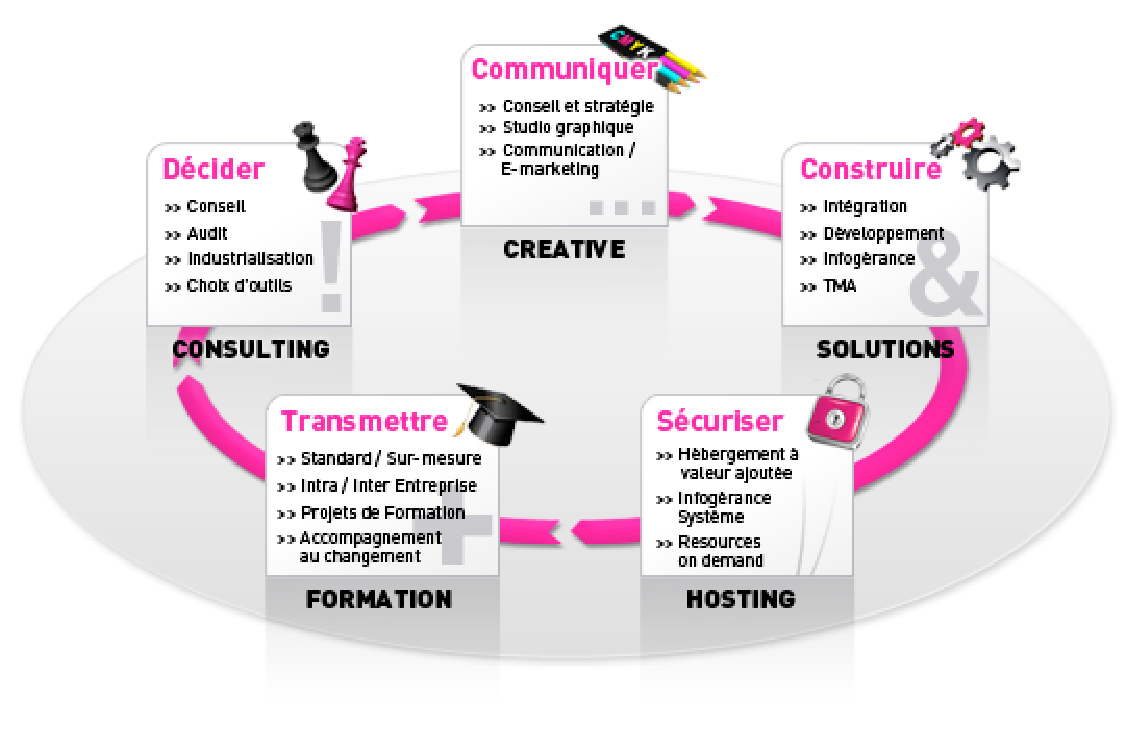
\includegraphics[width=0.9\textwidth]{resource/img/aw_360}
	\caption{Les différentes branches d'Alter Way}
	\end{figure}

\section{Histoire}
\paragraph*{}
	Créee en 2006, Alter Way est la première entreprise française à avoir fédéré les acteurs historique
	de l'open source autour d'un projet d'industrialisation du marché:

	\begin{description}
		\item[Anaska] Leader français de formation open source en 2001
		\item[Eclip's Software] Éditreur d'une solution d'administration réseau
		\item[Ingeniweb] Spécialiste en solution web d'entreprise de gestion de contenu
		\item[Kanopee] Consultants en développement PHP
		\item[Nexen Services] Hébergement et Infogérance LAMP\footnote{Linux Apache MySQL PHP}
		\item[O4DB] Expertise en BDD\footnote{Base de Donnée}
		\item[Solinux] Spécialistes dans l'administration de platforme Linux et l'intégration d'OpenXchange
	\end{description}

	Afin de renforcer son offre globale et de soutenir sa stratégie de développement sur le web, Alter Way
	a également intégré l'agence de communication \emph{Reciprok}, spécialisée en conseil en communication,
	studio graphique et web-marketing.

	\begin{figure}
		\centering
		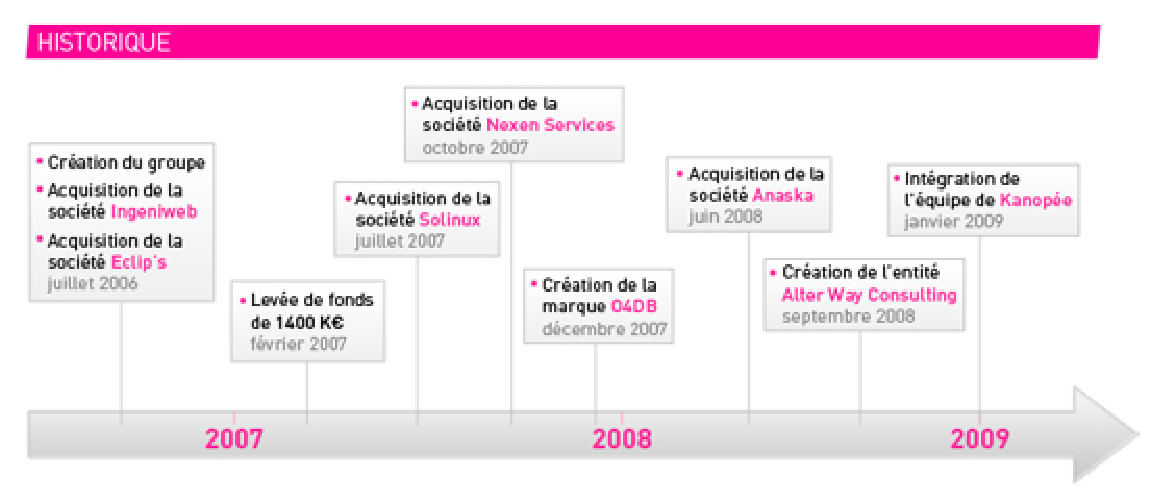
\includegraphics[width=0.9\textwidth]{resource/img/historique_aw}
		\caption{L'histoire d'Alter Way}
	\end{figure}

\section{Quelques chiffres (2010)}
	\begin{itemize}
		\item 10M\euro{} de Chiffre d'affaire
		\item 10\% de croissance
		\item Résultats: +4.5\%
		\item 120 collaborateurs
	\end{itemize}


\section{Alter Way Hosting}
\paragraph*{}
Alter Way Hosting (AWH) est la branche de la société dont le rôle est l'hébergement et l'infogérance de services internet.
Les services hébergés sont pour la plupart des sites web ainsi que des serveurs de messagerie.

\paragraph*{}
AWH est organisé en quatres équipes affectées à quatres types d'offres différentes:

\begin{description}
	\item[L'équipe responsable des serveurs dédiées vserveurs \footnotemark]
		\footnotetext{Technologie de virtualisation de système d'exploitation permettant d'héberger plusieurs clients sur un seul serveur}
	\item[L'équipe responsable des offres mutualisées
		\footnotemark] \footnotetext{Plusieurs sites internet sont hébergés sur un même serveur par un seul logiciel de serveur web}
	\item[Les RTC \footnotemark des architectures] \footnotetext{RTC: Responsable Chef de Compte, similaire à Chef de Projet}
		gèrent les clients les plus importants possédant plusieurs serveurs dédiés
	\item[Les responsable de l'infrastructure] s'occupent des tâches plus globale touchant à tout les serveurs,
		principalement la gestion du réseau.



\end{description}


